\documentclass[margin=2pt]{standalone}
\usepackage{tikz}

\begin{document}
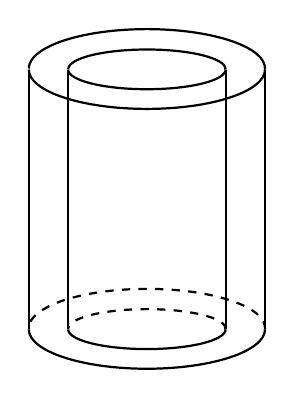
\begin{tikzpicture}
%cylinder
\draw [thick](-1.5,-1.65) -- (-1.5,1.65);
\draw [thick](+1.5,-1.65) -- (+1.5,1.65);
\draw [thick](-1.5,-1.65) arc (180:360:1.5 and 0.5);          % <--
\draw[thick,dashed] (1.5,-1.65) arc (-1.65:180:1.5 and 0.5);  % <--
\draw [thick](-1.5,+1.65) arc (180:360:1.5 and 0.5);          % <--
\draw [thick](+1.5,+1.65) arc (-1.5:180:1.5 and 0.5);         % <--
%\draw[thick,gray,dashed](0,-1.65) --(+1.5,-1.65);
%hollow
\draw [thick](-1,-1.65) -- (-1,1.65);
\draw [thick](+1,-1.65) -- (+1,1.65);
\draw [thick](-1,-1.65) arc (180:360:1 and 0.25);
\draw[thick,dashed] (1,-1.65) arc (-1.65:180:1 and 0.25);
\draw [thick](-1,+1.65) arc (180:360:1 and 0.25);
\draw [thick](+1,+1.65) arc (-1:180:1 and 0.25);
%\draw[thick,gray,dashed](0,-1.65) --(+1,-1.65);
%
%\fill[fill=black] (0,-1.65) circle (1.5pt);
%\node[below,scale=0.8] at (1.2,-2) {$R$};
%%
%% I changed a little the node position; removed \text{}
%% node for R_1 below
%\draw [thick,<->] (0,-1.5) -- node[fill=white,inner sep=1pt] {\scriptsize$R_1$} (1,-1.5);
%\draw [thick,<->] (0,-2.5) -- node[fill=white,scale=0.9,inner sep=1pt] {$0.5$ m} (1.5,-2.5);
%\draw [thick,<->] (2.1,1.65) -- node[fill=white,scale=0.9, inner sep=1pt] {$h$ cm} (2.1,-1.65);
\end{tikzpicture}
\end{document}